% !TEX encoding = UTF-8 Unicode
% -*- coding: UTF-8; -*-
% vim: set fenc=utf-8

\chapter{Experimentos}%
\label{chap:experimentos}

Esse capítulo apresentará alguns exemplos de experimentos e de simulações computacionais, que foram executados a fim de ilustrar a implementação do Query Processor --- apresentado no \autoref{chap:rastros-de-proveniencia} ---, assim como os resultados obtidos com os mesmos.

\perrotta{TODO: EXPAND}

\section{Simulação Computacional em Sedimentação}

% - referenciar supercomputing (SC 2016)

Todos os exemplos de consultas desse capítulo utilizam o mesmo fluxo de dados \(D^{\dagger}\) ilustrado na \autoref{fig:experiments-dataflow}.

\perrotta{Introdução}

\perrotta{Capítulo 06 --- Ilustrar o dataset de exemplo}

\begin{figure}[!htb]
    \centering
    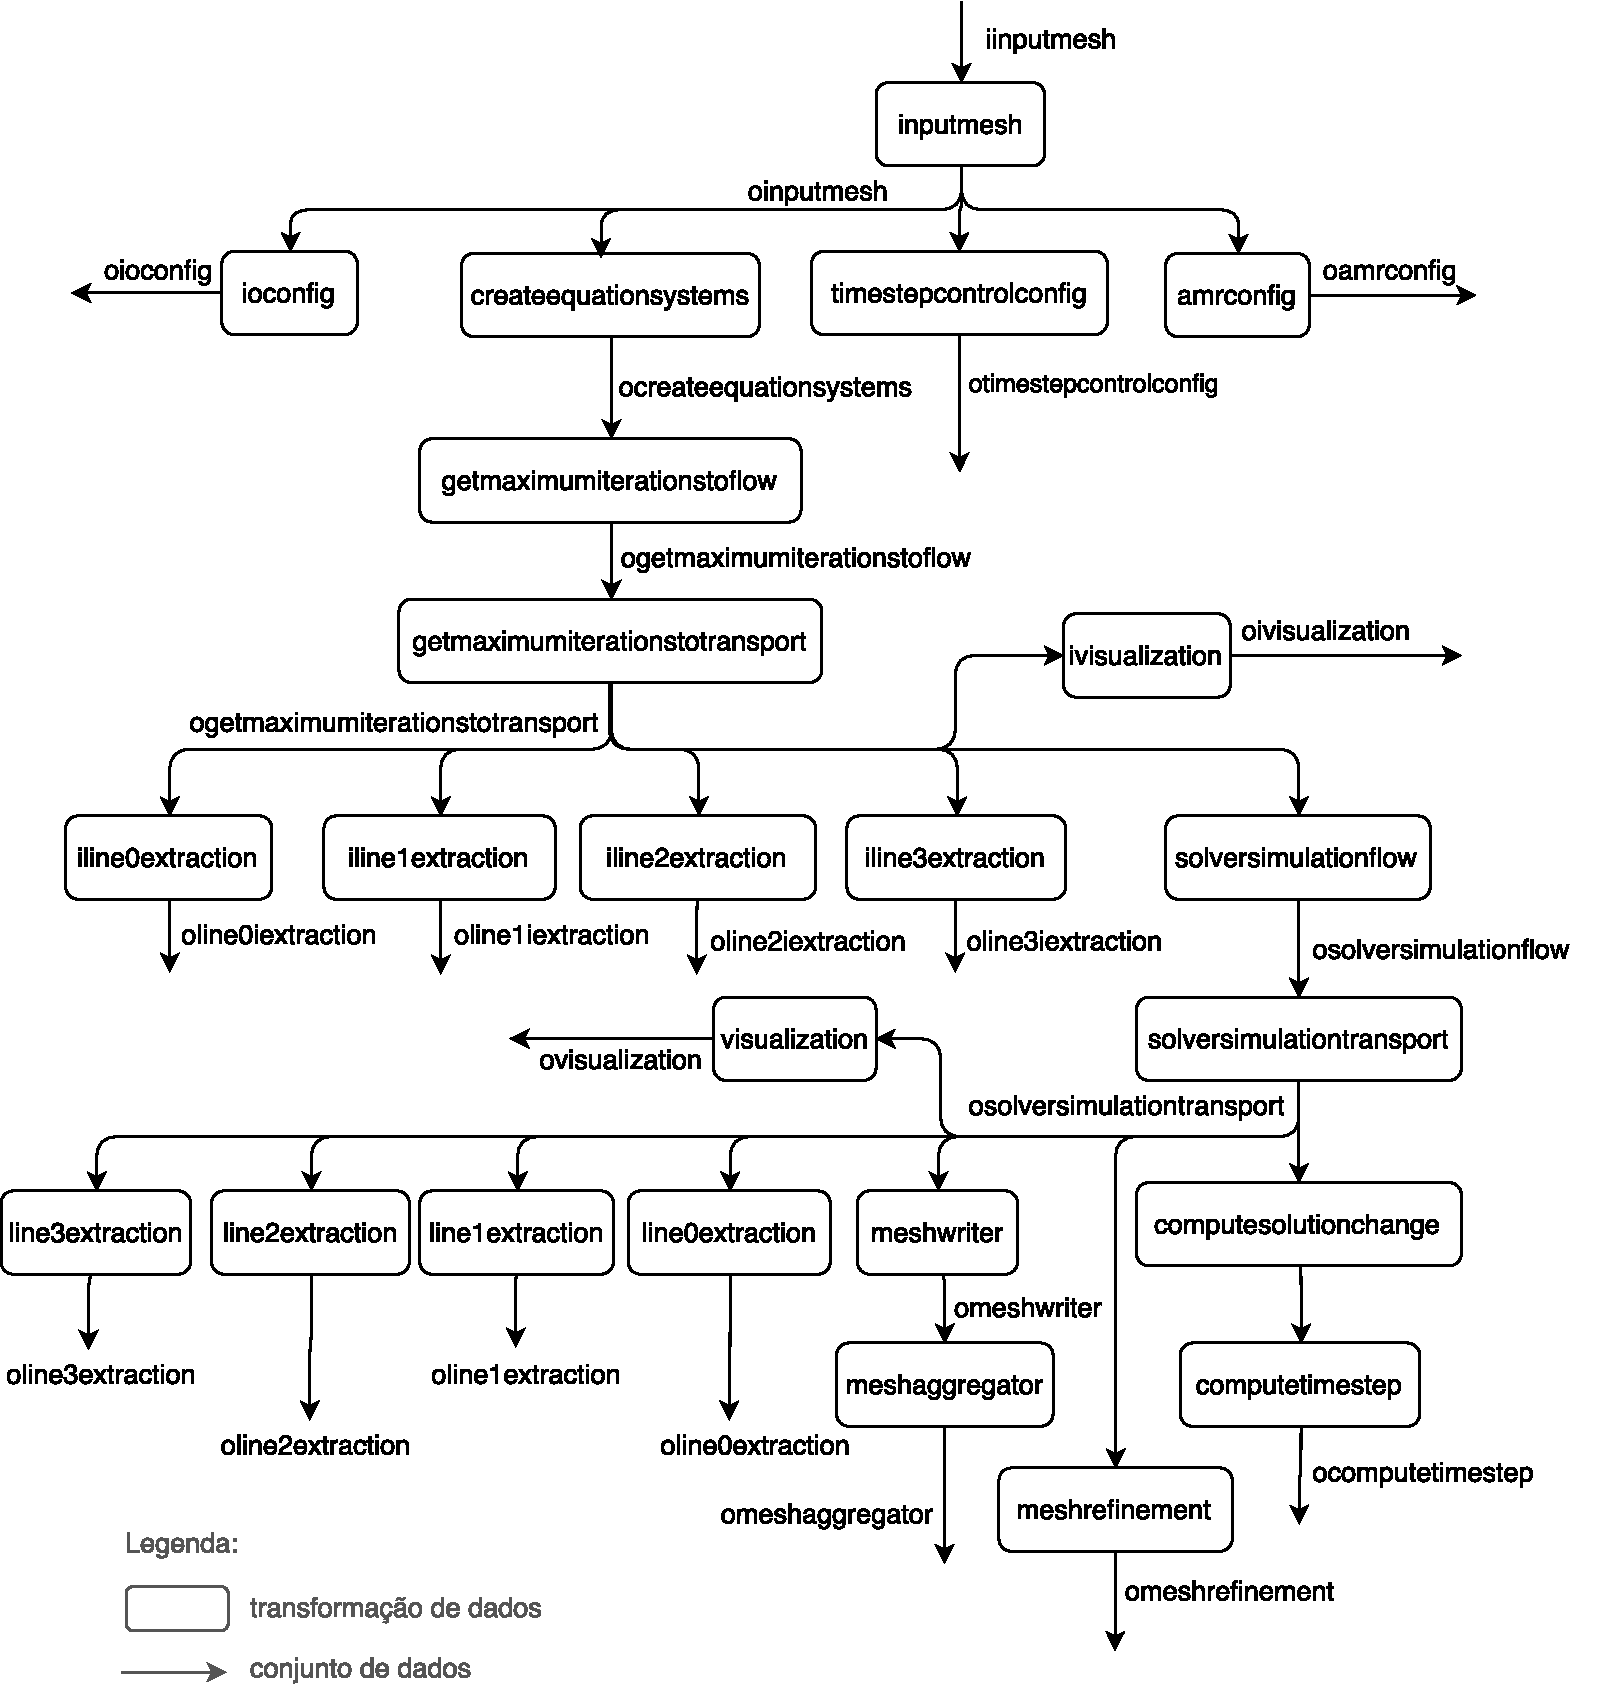
\includegraphics[width=\textwidth]{img/experiments-dataflow}
    \caption[Fluxo de dados $D^{\dagger}$ utilizado nos experimentos]{Fluxo de dados $D^{\dagger}$ utilizado nos experimentos e nas consultas do \autoref{chap:experimentos}.}%
    \label{fig:experiments-dataflow}
\end{figure}

\section{Experimentos}

Os experimentos relacionados ao Query Processor foram executados em um computador com as seguintes especificações:

\begin{itemize}
	\item Macbook Pro Retina 2015, com o sistema operacional macOS Sierra 10.12.6;
    \item Processador Intel Core i5 2,7~GHz, com 4~CPUs;
    \item 8~GB de memória RAM do tipo DDR3.
\end{itemize}

\subsection{Consulta \#1}

% Tempo: rodar 4 vezes, tirar a média das 3 últimas

\perrotta{TODO: observação: GROUP BY}

\begin{table}[htb]
    \centering
    \begin{tabular}{c|c}
\textbf{Argumento}          & \textbf{Valor} \\ \hline
\texttt{D}                  & $D^{\dagger}$ \\
\texttt{dsOrigins}          & \{\texttt{osolversimulationtransport}\} \\
\texttt{dsDestinations}     & \{\texttt{oline2extraction}, \texttt{omeshwriter}\} \\
\texttt{type}               & physical \\
\texttt{projections}        & \{\texttt{osolversimulationtransport.time}, \texttt{AVG(oline2extraction.d)}\} \\
\texttt{selections}         & \varnothing \\
\texttt{dsIncludes}         & \varnothing \\
\texttt{dsExcludes}         & \varnothing \\
    \end{tabular}
    \caption[Argumentos da função \texttt{generateSqlQuery} para a consulta \#1]{Especificação dos argumentos da função \texttt{generateSqlQuery} para a consulta~\#1.}%
    \label{tab:experiments-1-especificacao}
\end{table}

\begin{figure}[htb]
    \centering
    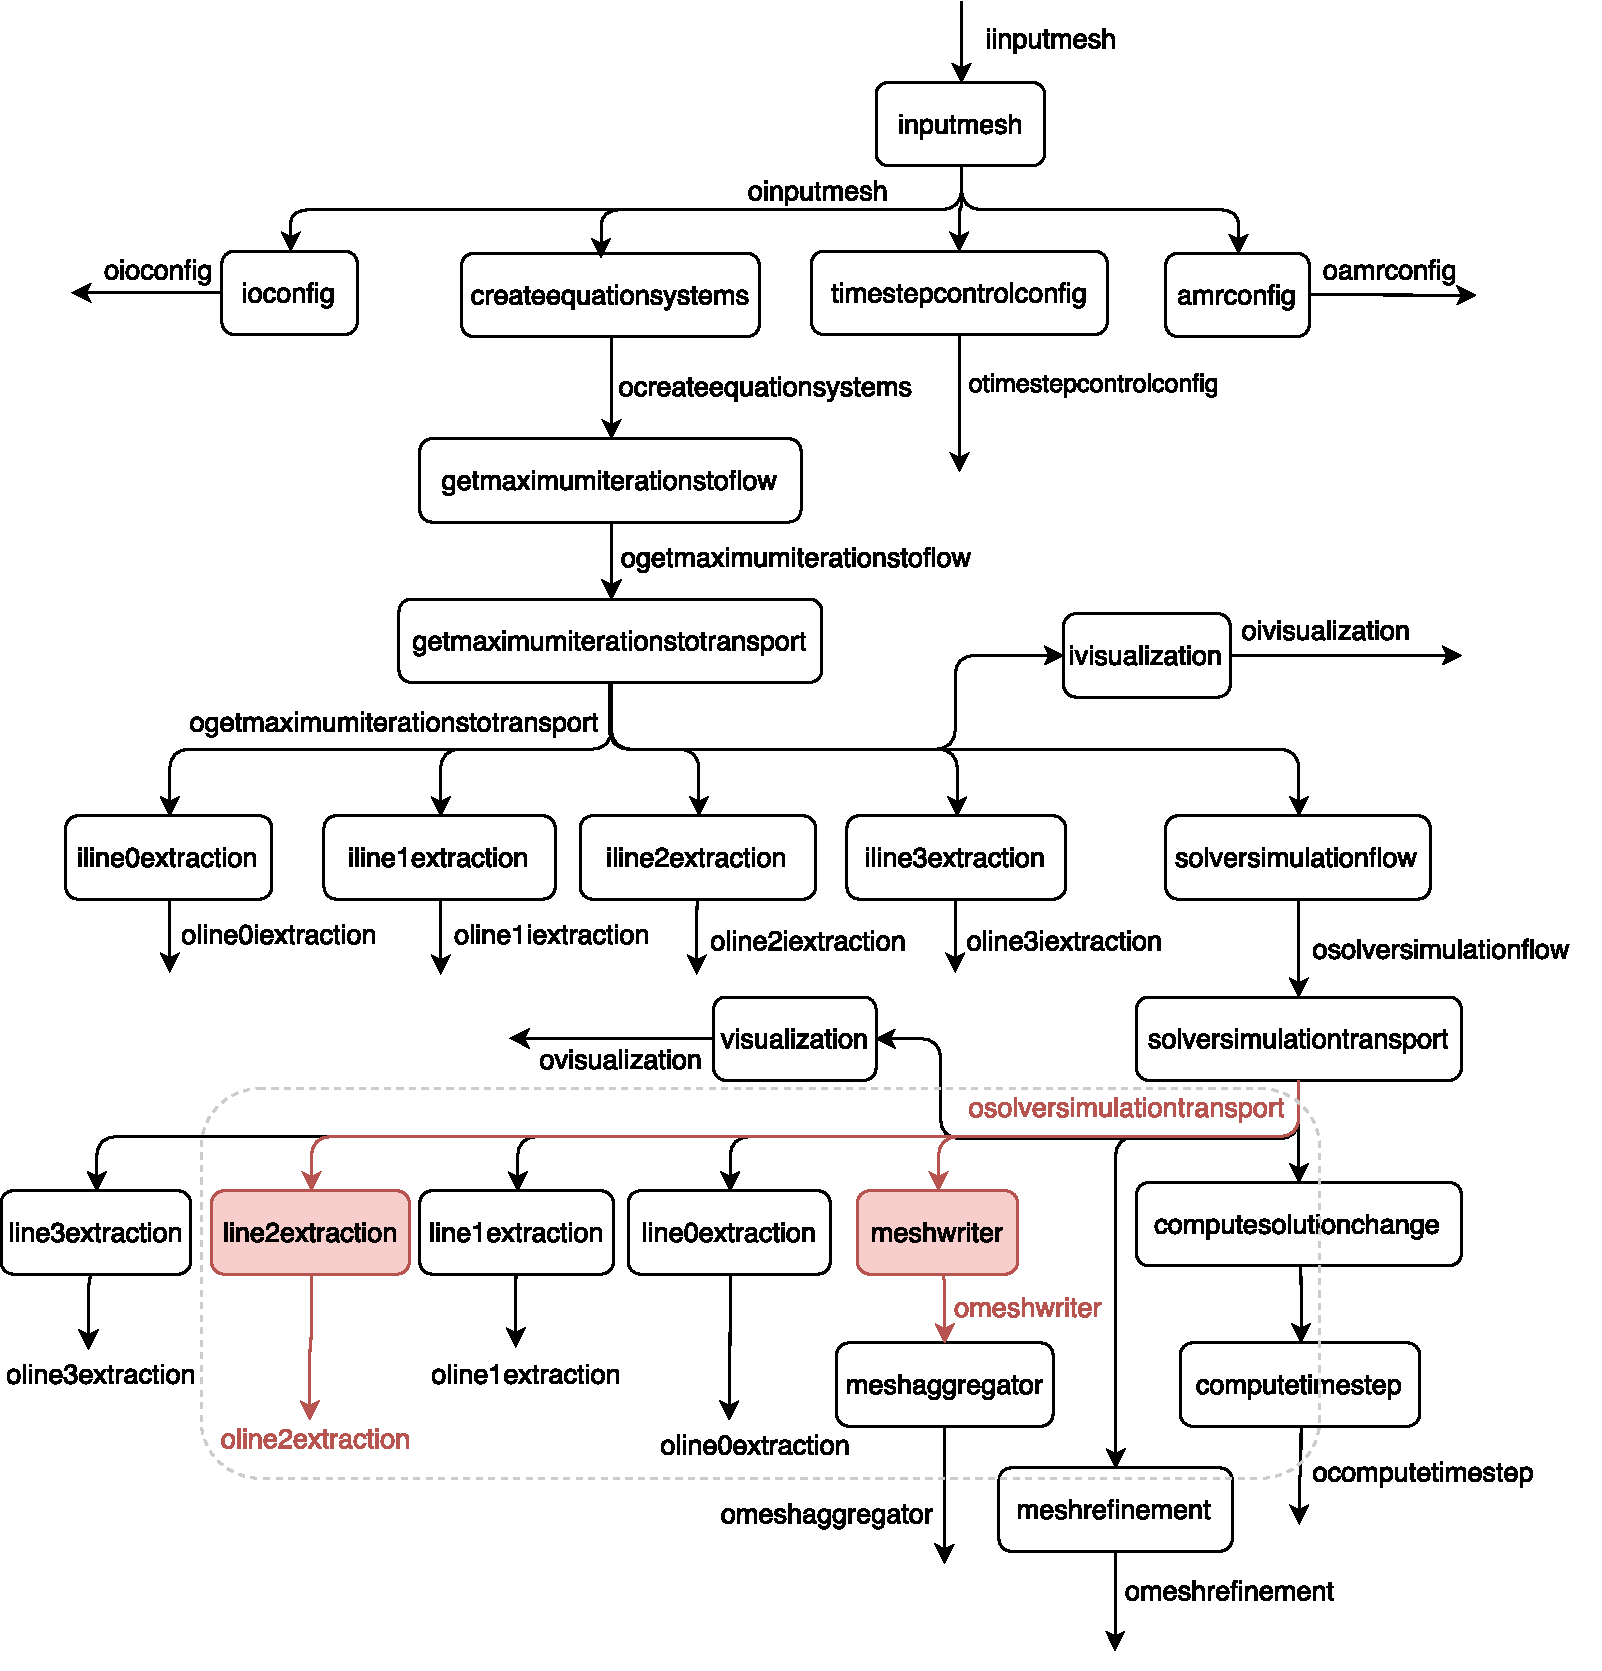
\includegraphics[width=\textwidth]{img/experiments-dataflow-1}
    \caption[Caminho do fluxo de dados \(D^{\dagger}\) rastreado na consulta \#1]{Caminho d fluxo de dados \(D^{\dagger}\) rastreado na consulta \#1.}%
    \label{fig:experiments-dataflow-1}
\end{figure}

\begin{minipage}[c]{0.95\textwidth}
\begin{lstlisting}[language=sql,label={lst:experiments-1-sql},caption={[Código em SQL gerado na consulta~\#1]Código em SQL gerado na consulta~\#1 (40,29~ms).}]
SELECT osolversimulationtransport.time, AVG(oline2extraction.d)
FROM osolversimulationtransport, oline2extraction, omeshwriter
WHERE (osolversimulationtransport.line2extraction_task_id = oline2extraction.line2extraction_task_id) 
AND (osolversimulationtransport.meshwriter_task_id = omeshwriter.meshwriter_task_id)
GROUP BY osolversimulationtransport.time;
\end{lstlisting}
\end{minipage}

\begin{minipage}[c]{0.95\textwidth}
\begin{lstlisting}[language=sqlresults,label={lst:experiments-1-sqlresults},caption={[Resultados da consulta \#1.]Resultados da consulta \#1 (7 tuplas, 4,346~ms).}]
+--------------------------+--------------------------+
| time                     | L71                      |
+==========================+==========================+
|                1.3398483 |     1.74129306930693e-44 |
|                3.1009347 |  -1.0847045643564339e-44 |
|                5.4124618 |    7.853749801980205e-39 |
|                7.8695609 |  -1.8180726336633645e-33 |
|               10.1307669 |   1.0729463267326738e-27 |
|               12.6055519 |   1.0473414950495052e-24 |
|                       15 |   -8.768540693069305e-22 |
+--------------------------+--------------------------+
\end{lstlisting}
\end{minipage}

\subsection{Consulta \#2}

\perrotta{TODO: observação: LIMIT 10}

\begin{table}[htb]
    \centering
    \begin{tabular}{c|c}
\textbf{Argumento}          & \textbf{Valor} \\ \hline
\texttt{D}                  & $D^{\dagger}$ \\
\texttt{dsOrigins}          & \{\texttt{osolversimulationtransport}\} \\
\texttt{dsDestinations}     & \{\texttt{oline0extraction}, \texttt{omeshwriter}\} \\
\texttt{type}               & physical \\ \hline
\texttt{projections}        & \makecell{\{\texttt{osolversimulationtransport.time}, \\
                                          \texttt{oline0extraction.points0}, \\ 
                                          \texttt{oline0extraction.points1}, \texttt{oline0extraction.points2}, \\
                                          \texttt{oline0extraction.d}\}} \\ \hline
\texttt{selections}         & \makecell{\{\texttt{osolversimulationtransport.time < 5.5}, \\
                                          \texttt{oline0extraction.d > 0.1}\}} \\ \hline
\texttt{dsIncludes}         & \varnothing \\
\texttt{dsExcludes}         & \varnothing \\
    \end{tabular}
    \caption[Argumentos da função \texttt{generateSqlQuery} para a consulta \#2]{Especificação dos argumentos da função \texttt{generateSqlQuery} para a consulta~\#2.}%
    \label{tab:experiments-2-especificacao}
\end{table}

\begin{figure}[htb]
    \centering
    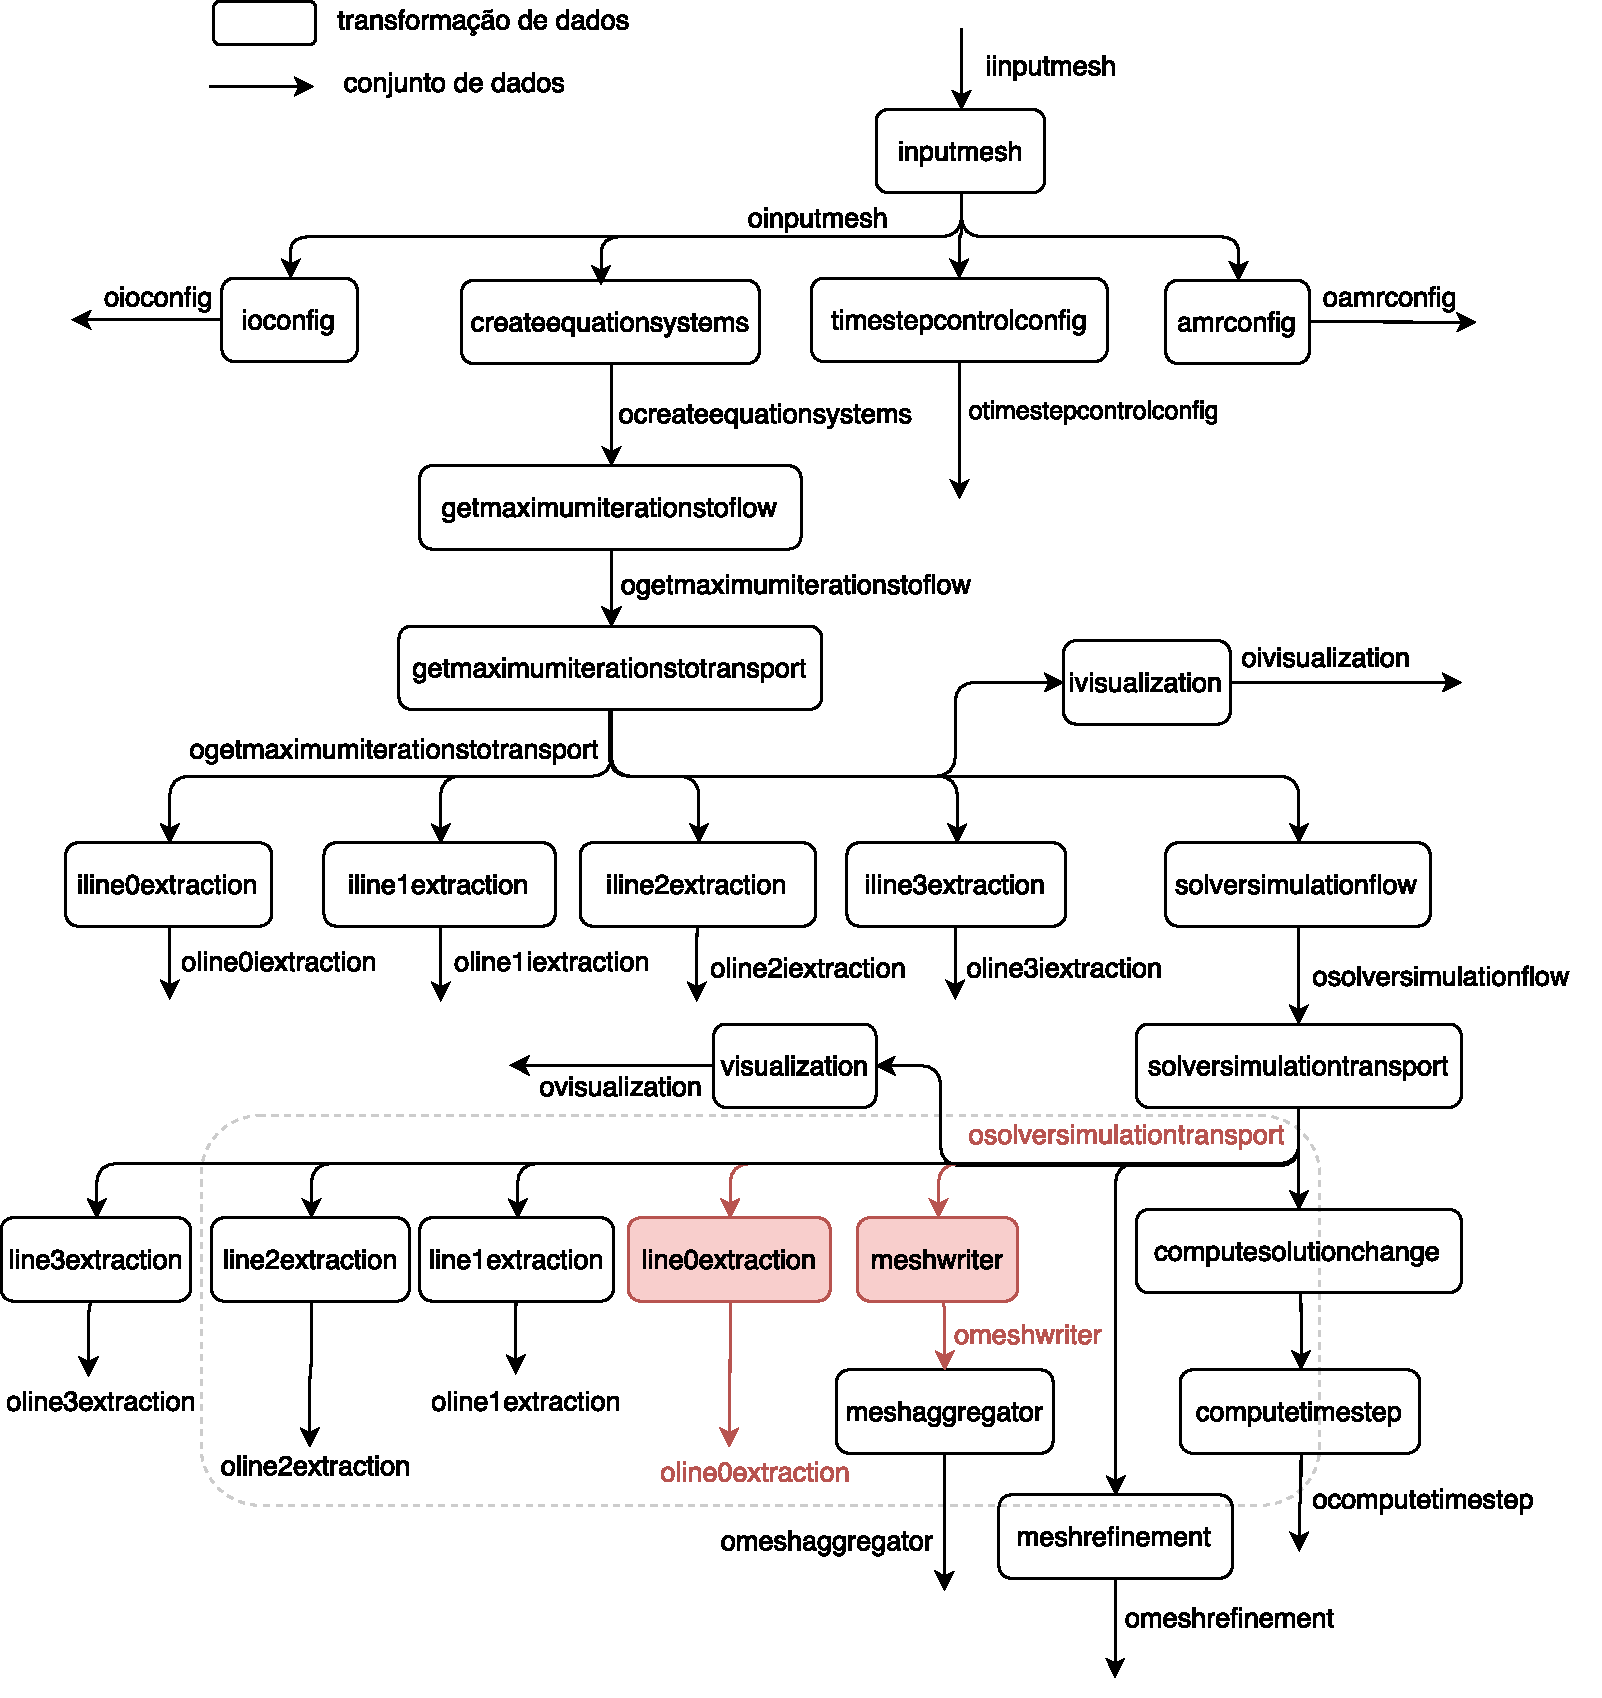
\includegraphics[width=\textwidth]{img/experiments-dataflow-2}
    \caption[Caminho do fluxo de dados \(D^{\dagger}\) rastreado na consulta \#2]{Caminho d fluxo de dados \(D^{\dagger}\) rastreado na consulta \#2.}%
    \label{fig:experiments-dataflow-2}
\end{figure}

\begin{minipage}[c]{0.95\textwidth}
\begin{lstlisting}[language=sql,label={lst:experiments-2-sql},caption={[Código em SQL gerado na consulta~\#2]Código em SQL gerado na consulta~\#2 (15,45~ms).}]
SELECT osolversimulationtransport.time, oline0extraction.points0, oline0extraction.points1, oline0extraction.points2, oline0extraction.d
FROM osolversimulationtransport, oline0extraction, omeshwriter
WHERE (osolversimulationtransport.time < 5.5) 
AND (oline0extraction.d > 0.1) 
AND (osolversimulationtransport.line0extraction_task_id = oline0extraction.line0extraction_task_id) 
AND (osolversimulationtransport.meshwriter_task_id = omeshwriter.meshwriter_task_id)
LIMIT 10;
\end{lstlisting}
\end{minipage}

\begin{minipage}[c]{0.95\textwidth}
\begin{lstlisting}[language=sqlresults,label={lst:experiments-2-sqlresults},caption={[Resultados da consulta \#2.]Resultados da consulta \#2 (10 tuplas, 5,92~ms).}]
+--------------+-----------+---------+---------+----------+
| time         | points0   | points1 | points2 | d        |
+==============+===========+=========+=========+==========+
|    5.4124618 |         0 |       1 |       0 |  0.10814 |
|    5.4124618 |      0.18 |       1 |       0 |   0.1082 |
|    5.4124618 |      0.36 |       1 |       0 |  0.10825 |
|    5.4124618 |      0.54 |       1 |       0 |  0.10825 |
|    5.4124618 |      0.72 |       1 |       0 |  0.10825 |
|    5.4124618 |         0 |       1 |       0 |  0.10814 |
|    5.4124618 |      0.18 |       1 |       0 |   0.1082 |
|    5.4124618 |      0.36 |       1 |       0 |  0.10825 |
|    5.4124618 |      0.54 |       1 |       0 |  0.10825 |
|    5.4124618 |      0.72 |       1 |       0 |  0.10825 |
+--------------+-----------+---------+---------+----------+
\end{lstlisting}
\end{minipage}

% |    5.4124618 |         0 |       1 |       0 |  0.10814 |
% |    5.4124618 |      0.18 |       1 |       0 |   0.1082 |
% |    5.4124618 |      0.36 |       1 |       0 |  0.10825 |
% |    5.4124618 |      0.54 |       1 |       0 |  0.10825 |
% |    5.4124618 |      0.72 |       1 |       0 |  0.10825 |
% |    5.4124618 |         0 |       1 |       0 |  0.10814 |
% |    5.4124618 |      0.18 |       1 |       0 |   0.1082 |
% |    5.4124618 |      0.36 |       1 |       0 |  0.10825 |
% |    5.4124618 |      0.54 |       1 |       0 |  0.10825 |
% |    5.4124618 |      0.72 |       1 |       0 |  0.10825 |

\subsection{Consulta \#3}

\perrotta{TODO: consulta \#3}

\subsection{Consulta \#4}

\perrotta{TODO: consulta \#4}